\documentclass[a4paper, 12pt]{article}

% a nice font
\usepackage{kpfonts}

% basic text stuff
\usepackage[utf8]{inputenc}
\usepackage[T1]{fontenc}

\usepackage{tikz} % main tikz package
\usepackage{pgfplots} % pgplots package

\pgfplotsset{
    compat = 1.17, % to have the same coordinate system between axis and draw
}

\usepackage{tikz-network} % provides graph / network utilities (Edge, Node, etc)


\usetikzlibrary{arrows.meta} % for nice arrows
\usetikzlibrary{calc} % to do some computations on the coordinates

% for a nicer colorscheme
%\definecolor{blue}{rgb}{0.38, 0.51, 0.71} %glaucous, 97,130,181, #6182B5
\definecolor{darkblue}{RGB}{17, 42, 60} % 112A3C
\definecolor{red}{RGB}{175, 49, 39} % AF3127

\definecolor{orange}{RGB}{217, 156, 55} % D99C37
\definecolor{green}{RGB}{144, 169, 84} % 90A954
\definecolor{palegreen}{RGB}{197, 184, 104} % C5B868

\definecolor{yellow}{RGB}{250, 199, 100} % FAC764
\definecolor{brokenwhite}{RGB}{218, 192, 166} % DAC0A6
\definecolor{brokengrey}{rgb}{0.77, 0.76, 0.82} % {196,194,209}, C4C2D1


\begin{document}

    % tangent plane formula from some stack exchange post
    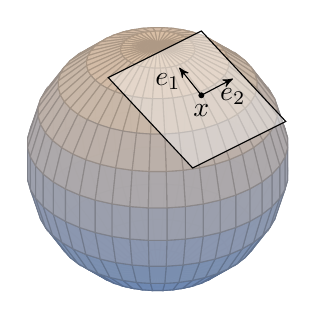
\begin{tikzpicture}[>=stealth',tangent plane/.style args={at #1 with vectors #2 and #3}{insert path={#1 --  ($#1+($#2-(0,0,0)$)$) --  ($#1+($#2-(0,0,0)$)+($#3-(0,0,0)$)$) -- ($#1+($#3-(0,0,0)$)$) -- cycle}}]
        \begin{axis}[%
            axis equal,
            hide axis,
            width=10cm,
            height=10cm,
            axis lines = center,
            xlabel = {},
            ylabel = {},
            zlabel = {},
            ticks=none,
            enlargelimits=0.3,
            colormap={whiteblue}{color=(blue) color=(white)},
            colormap={gb}{color=(green) color=(yellow)
                color=(brown)},
            view/h=45,
            scale uniformly strategy=units only,
        ]
        \addplot3[%
            opacity = 0.95,
            z buffer = sort,
            surf,
            samples = 23,
            variable = \u,
            variable y = \v,
            domain = 0:360,
            y domain = 0:180,
            colormap={slategraywhite}{rgb255=(97,130,181) rgb255=(218, 192, 166)},
        ]
        ({sin(u)*cos(v)}, {sin(u)*sin(v)}, {cos(u)});

        \draw[fill=white,fill opacity=0.4,
            tangent plane=at {({cos(65)-0.5*sin(65)},-0.5,{sin(65)})} with 
            vectors {({sin(65)},0,{-cos(65)})} and {(0,1,0)}];

        \end{axis}

        % I used trial and errors to find nice coordinates for those next nodes
        \coordinate (x) at (4.3,5);

        \draw[fill] (x) circle (0.03) node[below] {$x$};

        \draw[->] (x) to node[left] {$e_1$} (4.02,5.35) ;
        \draw[->] (x) to (4.7,5.21) node[below] {$e_2$};

    \end{tikzpicture}
\end{document}
